\documentclass[tikz,border=12pt]{standalone}
\usepackage[T1]{fontenc}
\usepackage[utf8]{inputenc}
\usepackage{lmodern}
\usetikzlibrary{arrows.meta}

% Evolução coordenada do gêmeo digital (DSQ) e do sistema real (RSQ).
% Arquivo independente: compile com pdflatex ou envie ao Overleaf.
\definecolor{ink}{HTML}{25344A}
\definecolor{muted}{HTML}{617287}
\definecolor{blueband}{HTML}{E8F2FA}
\definecolor{blueborder}{HTML}{3B78AA}
\definecolor{yellowband}{HTML}{FFF3D7}
\definecolor{yellowborder}{HTML}{C98A28}
\definecolor{redband}{HTML}{F9E9EA}
\definecolor{redbox}{HTML}{AF343B}

\tikzset{
  stage/.style={
    rectangle, rounded corners=4pt, draw=ink!55, fill=white,
    line width=0.8pt, text width=2.42cm, minimum height=1.15cm,
    align=center, inner xsep=5pt, inner ysep=5pt,
    font=\small
  },
  digital/.style={stage, draw=blueborder!80},
  real/.style={stage, draw=yellowborder!85},
  evolution digital/.style={-{Latex[length=2.5mm]}, draw=blueborder,
    line width=1.15pt, line cap=round},
  evolution real/.style={-{Latex[length=2.5mm]}, draw=yellowborder,
    line width=1.15pt, line cap=round},
  guidance/.style={-{Latex[length=2.4mm]}, draw=muted,
    line width=0.9pt, dashed},
  outcome link/.style={-{Latex[length=2.4mm]}, draw=redbox!80,
    line width=1pt, line cap=round}
}

\begin{document}
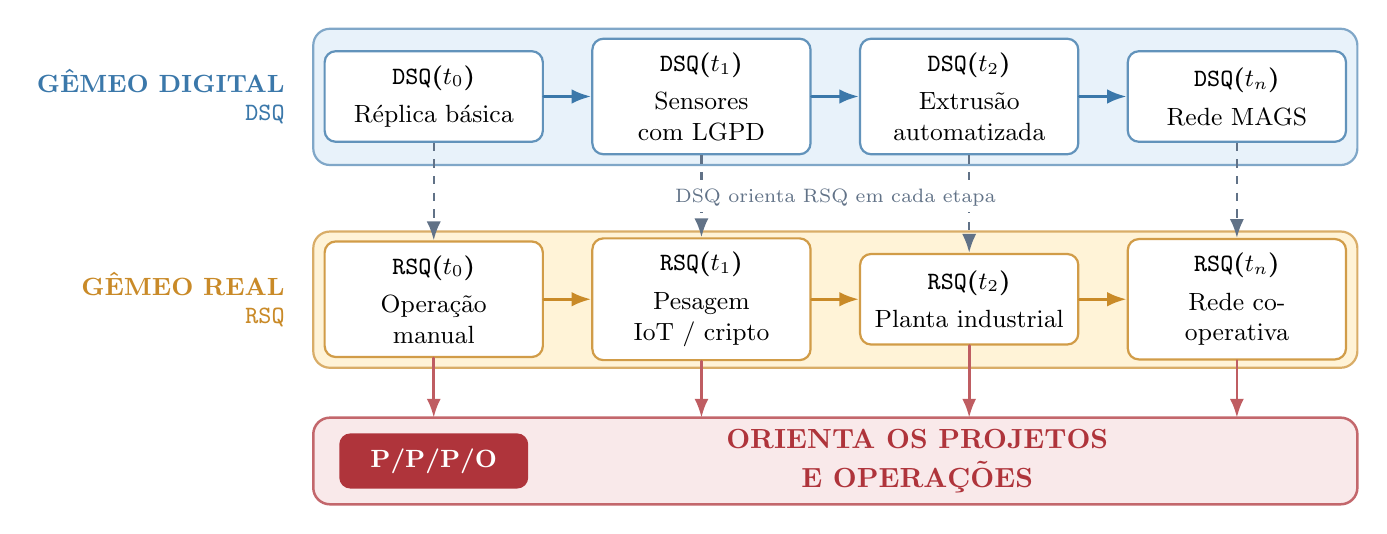
\begin{tikzpicture}[font=\sffamily]

  % Cabeçalho e faixas.
  % [comentado a pedido: título e subtítulo removidos da figura]
  % \node[font=\bfseries\Large, text=ink] at (5.1,8.25)
  %   {Evolução coordenada DSQ--RSQ};
  % \node[font=\small, text=muted] at (5.1,7.76)
  %   {Quatro estados ao longo do tempo};

  \filldraw[fill=blueband, draw=blueborder!65, line width=0.8pt,
            rounded corners=6pt]
    (-1.53,5.47) rectangle (11.73,7.20);
  % Faixa amarela: gap azul->amarelo aumentado +15% (0.735 -> 0.845).
  \filldraw[fill=yellowband, draw=yellowborder!70, line width=0.8pt,
            rounded corners=6pt]
    (-1.53,2.895) rectangle (11.73,4.625);

  % Títulos de trilha fora das faixas, sem cruzar as setas verticais.
  \node[anchor=east, align=right, text=blueborder, font=\bfseries\small]
    at (-1.77,6.34) {GÊMEO DIGITAL\\[-1pt] \normalfont\texttt{DSQ}};
  \node[anchor=east, align=right, text=yellowborder, font=\bfseries\small]
    at (-1.77,3.765) {GÊMEO REAL\\[-1pt] \normalfont\texttt{RSQ}};

  % Estados alinhados por tempo.
  \node[digital] (d0) at (0,6.34)
    {{\bfseries\texttt{DSQ}($t_0$)}\\[3pt] Réplica básica};
  \node[digital] (d1) at (3.4,6.34)
    {{\bfseries\texttt{DSQ}($t_1$)}\\[3pt] Sensores com LGPD};
  \node[digital] (d2) at (6.8,6.34)
    {{\bfseries\texttt{DSQ}($t_2$)}\\[3pt] Extrusão automatizada};
  \node[digital] (dn) at (10.2,6.34)
    {{\bfseries\texttt{DSQ}($t_n$)}\\[3pt] Rede MAGS};

  % Linha RSQ: desce 0.11 para acompanhar a faixa amarela (gap +15%).
  \node[real] (r0) at (0,3.765)
    {{\bfseries\texttt{RSQ}($t_0$)}\\[3pt] Operação manual};
  \node[real] (r1) at (3.4,3.765)
    {{\bfseries\texttt{RSQ}($t_1$)}\\[3pt] Pesagem IoT / cripto};
  \node[real] (r2) at (6.8,3.765)
    {{\bfseries\texttt{RSQ}($t_2$)}\\[3pt] Planta industrial};
  \node[real] (rn) at (10.2,3.765)
    {{\bfseries\texttt{RSQ}($t_n$)}\\[3pt] Rede cooperativa};

  % Setas horizontais = avanço temporal em cada trilha.
  \draw[evolution digital] (d0.east) -- (d1.west);
  \draw[evolution digital] (d1.east) -- (d2.west);
  \draw[evolution digital] (d2.east) -- (dn.west);
  \draw[evolution real] (r0.east) -- (r1.west);
  \draw[evolution real] (r1.east) -- (r2.west);
  \draw[evolution real] (r2.east) -- (rn.west);

  % Setas verticais tracejadas = orientação DSQ -> RSQ em cada etapa.
  % (uso .south/.north dos nós: acompanham sozinhas o novo espaçamento)
  \draw[guidance] (d0.south) -- (r0.north);
  \draw[guidance] (d1.south) -- (r1.north);
  \draw[guidance] (d2.south) -- (r2.north);
  \draw[guidance] (dn.south) -- (rn.north);
  % Rótulo recentralizado no novo vão (maior) entre as faixas azul e amarela.
  \node[fill=white, inner xsep=5pt, inner ysep=2pt,
        text=muted, font=\scriptsize]
    at (5.1,5.05) {DSQ orienta RSQ em cada etapa};

  % Faixa de desdobramento: gap amarelo->vermelho reduzido -35%
  % (0.975 -> 0.634). Toda a faixa vermelha e seu conteúdo sobem 0.231.
  \filldraw[fill=redband, draw=redbox!75, line width=0.9pt,
            rounded corners=6pt]
    (-1.53,1.161) rectangle (11.73,2.261);
  \foreach \r/\x in {r0/0,r1/3.4,r2/6.8,rn/10.2}
    \draw[outcome link] (\r.south) -- (\x,2.261);

  \node[fill=redbox, text=white, rounded corners=4pt,
        minimum width=2.40cm, minimum height=0.70cm,
        font=\bfseries\small] at (0,1.711) {P/P/P/O};
  \node[text=redbox, align=center, font=\bfseries\normalsize]
    at (6.14,1.711) {ORIENTA OS PROJETOS\\[2pt] E OPERAÇÕES};

\end{tikzpicture}
\end{document}